This chapter will give an overview of the main research questions for this project and how I intend to investigate them.

\section{Aspect classification schema}
One inherent drawback of computational methods is exactly their one unifying characteristic: their computability. Sadly, the requirement for computability means, in many cases, sacrificing the nuance that comes with more qualitative approaches. In this concrete case this means settling for a single aspect classification system. 

A consequence of the glut of literature in the field is a glut of classification systems to go with it, each with their own idiosyncrasies and each having their own advantages and drawbacks. The classification schema I decided on was the schema designed as part of Uniform Meaning Representation (UMR) \citep{umr}, for several reasons. On the one hand, the schema was designed for ease of annotation and usability and thus does away with a lot of the theoretical baggage of other classification systems (such as the insistence on lexical aspect types). On the other hand, UMR provides a lattice for annotation (see \ref{fig:umr_aspect_tree}) meaning the level of the annotation classes can be adjusted to the needs of the annotation context, thus giving more flexibility. Furthermore, the schema is part of a larger framework, and hence a classification system using these labels has a practical application too, since, if it works well, it can be later integrated into a larger UMR parsing system.

\subsection{UMR}
\label{sect:umr}
UMR \citep{umr} was introduced in order to expand and further generalise the attempt to design an abstract semantic representation, as was most successfully pioneered by \citet{amr} with Abstract Meaning Representation (AMR). In contrast to AMR, UMR aims to be a typologically-informed abstraction away from English structures, making it more suitable for other similar languages, or, in their own words, making it "a practical and cross-linguistically valid meaning representation designed to meet the needs of a wide range of NLP applications" \citep{umr}.

ADD STUFF HERE ABOUT HOW UMR WORKS GENERALLY
- SENTENCES AS GRAPHS (NODES + EDGES)
- SENTENCE LEVEL and DOC LEVEL
- EXAMPLE GRAPH

\subsection*{Aspect in UMR}
\label{aspect_in_umr}
UMR describes the following 5 coarse-grained aspect classes (descriptions adapted from \citet{umr} and the \href{https://github.com/umr4nlp/umr-guidelines/blob/master/guidelines.md}{UMR annotation guidelines}), also depicted in figure \ref{fig:umr_aspect_tree}:
\begin{itemize}
    \item \textbf{state} - stative events, i.e. no change takes place over the course of the event
    \item \textbf{habitual} - an event that occurs regularly in the past or
    present, including generic statements
    \item \textbf{activity} - an event that has not necessarily ended and may
    be ongoing at Document Creation Time\footnote{Since UMR was mostly designed for written text, they use the creation time of the document as a reference point. In spoken language this could be equated with time of utterance, though slightly different, since speech is an extended act, whereas document publication is punctual.} (DCT)
    \item \textbf{endeavour} - a process that ends without reaching its result state
    (i.e., termination)
    \item \textbf{performance} - a process that ends reaching its result state
\end{itemize}

\begin{figure}
    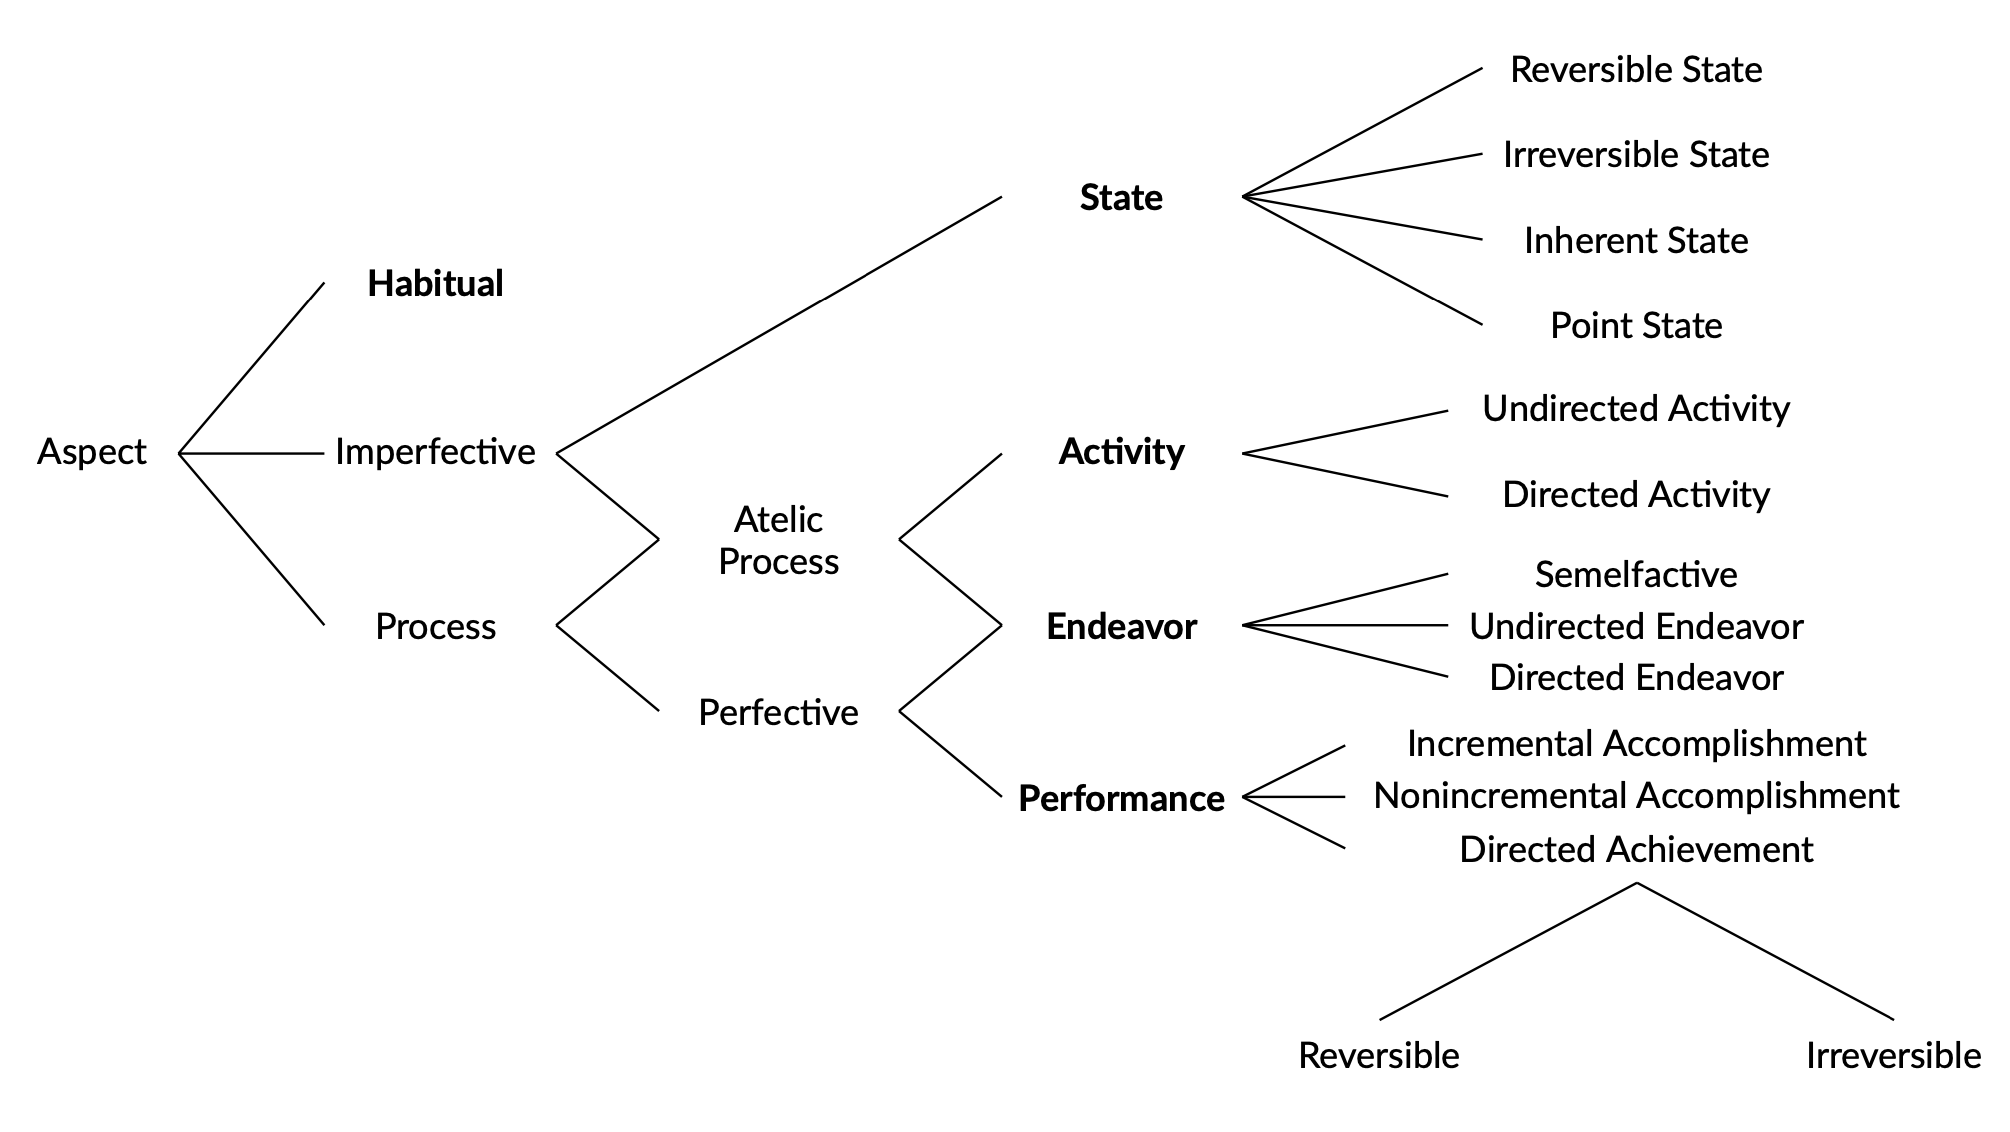
\includegraphics[width=\textwidth]{img/umr_aspct_tree.png}
    \caption{UMR aspect classification lattice \citep{umrslides2022}}
    \label{fig:umr_aspect_tree}
\end{figure}

How these relate to other aspectual classification schemata can be seen in table \ref{table:aspect_classes_comparison}.

Interesting to note is that these classes conflate the distinction made earlier between lexical and grammatical aspect, most clearly in the class "habitual", which is (in almost all cases) a paradigmatic example of an outer aspect, rather than one inherent in the verb event itself. Therefore, as can be seen in figure \ref{fig:umr_aspect_tree}, while classes which would usually be seen as grammatical aspect are to be found nearer the top of the tree (on the left), the leaves further down the tree are more examples of \emph{Aktionsarten}. That \citet{umr} make no mention of these different types of aspect is not necessarily surprising, given one of the main design goals of UMR is scalability, which entails learnability for annotators. As already mentioned, the theoretical distinction of inner and outer aspect is "very difficult to apply in practice" \citep{Dahl1985TenseAA}, hence a clear separation would often be difficult - and indeed not very fruitful - for annotators. Furthermore, this conflation of two phenomena can also be an advantage, since it shows the relationship between classes of each type (i.e. that \emph{irreversible states} are imperfective and \emph{directed achievements} perfective etc.), subsuming them all into \emph{one} semantic parameter space concerning aspect.

\begin{table}[]
    \begin{adjustbox}{width=\textwidth}
    \begin{tabular}{|l|l|l|l|l|l|l|}
    \hline
    \citet*{vendler57} &  \citet*{moens-steedman-1988-temporal}& \citet*{egg2005flexible} & \multicolumn{3}{l}{\citet*{annotAndAutoClassOfAspectCat}}  \vline & \citet{umr} \\ \hline \hline
\multirow{2}{*}{state}         & state                      & stative predicate     & \multicolumn{3}{l}{stative} \vline & \textbf{state} \\ \cline{2-7}
                               & (habitual state)           & (CHECK THIS)          & \multicolumn{3}{l}{-} \vline & \textbf{habitual} \\ \hline
activity                       & \multirow{2}{*}{process}   & process predicate     & \multirow{5}{*}{dynamic} & \multicolumn{2}{l}{unbounded} \vline & \textbf{activity} \\ \cline{1-1}\cline{3-3}\cline{5-7}
\multirow{2}{*}{accomplishment}&                            & intergressive predicate&      & \multirow{4}{*}{bounded} &  extended/no change & \textbf{endeavour} \\ \cline{2-3}\cline{6-7}
                               & culminated process         & change predicate      &       &  & extended/change & \textbf{performance}\\ \cline{1-3}\cline{6-7}
\multirow{2}{*}{achievement}   & point                      & intergressive predicate&      &  & punctual/no change & \textbf{endeavour} \\ \cline{2-3} \cline{6-7}
                               & culmination                & change predicate      &       &  & punctual/change & \textbf{performance} \\ \hline

    \end{tabular}
    \end{adjustbox}
    \caption{(Approximate) Comparison of aspectual classes. Adapted and extended from \citet*{annotAndAutoClassOfAspectCat}.}
    \label{table:aspect_classes_comparison}
\end{table}

\subsection*{Difficulties with aspect in UMR}
The UMR aspect system does come with some difficulties. Firstly, the classification scheme is notably different from those that came before it, since it is neither based on Vendler's classification, nor on typical binary aspect parameters, but rather seeks to create a typologically-informed aspect classification, taking into account explicit aspect encoding systems from a variety of languages. For example, the highest distinction made by \citet{comrie1976aspect} was between \textsc{perfective} and \textsc{imperfective}, while in UMR there are classes such as \textsc{endeavor} which can be both. The independence from the classic aspect parameters such as \textsc{telicity} or \textsc{durativity} also means the datasets annotated for one of these parameters cannot be easily used.

Secondly, UMR and its annotation guidelines are relatively new, hence sometimes unclear and are subject to change. This means that there are currently some minor inconsistencies between the annotated data available and the guidelines are sometimes unclear or problematic. I hope that as the project grows and expands to other languages, the annotation guidelines will be revised and refined and the inconsistencies fewer. At time of writing,\footnote{June 2024} the version 1.0 of the annotation guidelines has not yet been released.
\section{Research questions}
This section describes the research questions which the following study aims to answer.
\subsection*{RQ1: Can we train a system to identify aspect classes?}
The first question I aim to look at is whether we can train a system to automatically classify verbs in context as one of several aspect classes. This has been done before (see \ref{sect:previous_asp_class}), however this is the first time, to the best of my knowledge, that a \emph{large} language model\footnote{Defined as having > 1 million parameters, compared to BERT's 345 million.} has been used for this task. If this model works well, it will be possible to use it to look at some linguistic questions, such as whether particular prefixes in Slavic languages tend towards certain aspect classes, or carrying out a typological analysis of aspectual ambiguity (RQ3). 
\subsection*{RQ2: Can we automatically identify aspectually ambiguous verbs/sentences and which classes they tend towards?}
Once I have a model which can accurately predict verbal aspect in context, the next question will be the more complex task of predicting aspectual ambiguity. At this stage it is also an interesting question to examine how verb phrases are classified without context. This could shed some light on inherent aspectual readings of verb phrases and thus answer the question of whether there are some verb phrases which are perhaps "underspecified" in the model's latent space (see \ref{sect:coerc_or_under}).
\subsection*{RQ3: How does aspectual ambiguity compare across languages? Can we study the typology of aspectualisation?}
Finally, I will attempt to investigate and compare aspectual ambiguity across languages, looking at whether languages with more explicit marking for aspect have less aspect ambiguity than those expressing aspect more implicitly. I plan to answer this both by looking at the ambiguity classification of verbs in context and also of the top \emph{n} verbs in languages without context.
\section{Project outline}
\subsection*{Step 1: Fine-tune LLM for aspect classification}
In order to use language models to investigate aspect, it is necessary to first understand how much current language models know about aspectual phenomena. To this end, I will fine-tune a large language model on a small dataset (since no large datasets are available for the aspect classification scheme I choose, UMR \citep{umr}, or indeed in general for an aspect classification task), testing on a hold-out set. This step of fine-tuning a \emph{large} language model is necessary due to the scarcity of data available, which is not sufficient for fine-tuning a smaller model.
\subsection*{Step 2: Use fine-tuned LLM to annotate larger dataset}
The LLM fine-tuned in step 1 can then be used to annotate a larger dataset. Having a larger dataset allows a lot more possibilities for analysis than the dataset used for fine-tuning the larger model. For instance, this larger dataset can be used in a knowledge distillation (KD) process to train a smaller (possibly multilingual) model, which is useful for latent space analysis or comparison across languages. Though it must be noted that there is a danger of error propagation at this step.
\subsection*{Step 3: Compare aspectual systems cross-lingually}
Once we have training data of good enough quality, we can use this to train a multilingual model and use this to compare between languages. Here we can test the model in different contexts and use this to gain insights about the aspect systems of different languages, both in their own right and in comparison with one another, for example, to see if prevalence of aspectual ambiguity changes depending on how overtly a language marks for aspect, or if certain prefixes in a language mark a particular aspect class.

\subsection*{Step 4: Fine-tune LLM for aspect ambiguity detection}
In order to look at aspect ambiguity specifically, I will also fine-tune an LLM in a similar way to above to identify whether a verb in context has an ambiguous aspectual reading or not. However, since there does not yet exist a dataset annotated for aspectual ambiguity,\footnote{Recall that \citet{Friedrich2014AutomaticPO} only annotate ambiguity in the \textsc{dynamic/stative} parameter.} this part requires human annotation. I propose to solve this by requiring annotators to label sentence-verb pairs with any labels they see plausible. This makes it possible to have both a human class annotation and a derived ambiguity annotation for datapoints labelled with several labels. Neural networks are known for being overly confident in their predictions, and I will investigate whether low certainty of the smaller aspect \emph{classification} model (i.e. similar logit values across classes) correlates with the output of the model specially trained for ambiguity recognition.

\section{Use of LMs as sources of linguistic knowledge: Reversing the NLP pipeline}
One of the aims of this thesis is to highlight how language models can possibly be useful as sources of linguistic knowledge too. This idea is by no means new, and yet in the wider linguistics community outside computational linguistics, these tools seem to be little used.

Currently, the two main approaches used to develop and validate linguistic hypotheses are through corpora and through introspection, the former being championed by empiricists and the latter by the Chomskyan rationalist tradition \citep{corpus_textbook}. It is clear that corpora, including those used to train LLMs, can only contain a fraction of the famously infinite set of possible grammatical sentences in a language, and this has led Chomsky to decry corpus linguistics as seeking to model language \emph{performance} rather than \emph{competence} \citep{corpus_textbook}. Native speaker introspection, on the other hand, while able to judge the grammaticality of any sentence, is clearly highly subjective and biased. Language models, however, are productive and are able to generalise across their corpora to produce, with some sophistication, sentences not seen before in training, thus blurring the line between the traditional Chomskyan distinction between competence and performance.

While in the past, the NLP pipeline used to be made up of a host of linguistically informed steps (such as lemmatisation, dependency parsing and POS tagging), this changed with the advent of transformer models, which, some have argued, "rediscover" the classical NLP pipeline, albeit implicitly \citep{tenney2019bert}. Since these end-to-end models no longer require explicit linguistic encoding, one could argue that the importance of linguistic knowledge in NLP has dramatically decreased \citep{Church2021}, though it is undoubtedly true that linguistics is very useful for some areas of NLP which are currently less deep-learning inclined, such as low-resource NLP or meaning representation. Whether or not linguistics has a future in NLP, in this study I wish to look at the other direction of information flow and show that the benefits of collaboration between linguistics and NLP are not a one-way street.

\subsection*{When can (L)LMs \emph{not} help us?}
However, in light of the current hype surrounding deep learning it is important to highlight the limitations of such techniques and what language models \emph{cannot} do. 

It is well-known that training the LMs discussed in this paper requires a large amount of data and computing resources. While pre-trained models mean that LMs trained on relatively large amounts of data are now available for general use, for less well-resourced languages finding datasets of the necessary order of magnitude is a problem, and their performance suffers drastically. While this does not rule out the use of LMs on such languages (see \citep{kholodna2024llms}), it certainly limits the applicability and validity of some of the experiments described in this thesis to less well-resourced languages.

Furthermore, it must also be noted that LMs take on any biases present in the training data, meaning the language they approximate should be treated with caution. Examining these biases, as has often been done before, can, however, be an area of study in its own right and can produce valuable data for sociolinguistics. However, it must also be noted that it cannot be guaranteed that characteristics of a model's latent space can be transferred to a more general linguistic space, since human linguistic competence and LM competence differ in some aspects. Further research is therefore needed in this area.

Finally, since LMs are trained to minimize error on one variety of a language, they are less well-suited to study linguistic variation, whether geographical or temporal. This makes their use less suitable for languages without an accepted standard variant, such as Swiss German. In these cases, however, an approach using word embeddings with added dimensions such as \citet{hamilton-etal-2016-diachronic} could still be useful.